\documentclass[11pt,landscape]{article}
\usepackage{multicol}
\usepackage{calc}
\usepackage{ifthen}
\usepackage[landscape]{geometry}
\usepackage{hyperref}
\usepackage{amsmath}
\usepackage{graphicx}
\usepackage{float}

% To make this come out properly in landscape mode, do one of the following
% 1.
%  pdflatex latexsheet.tex
%
% 2.
%  latex latexsheet.tex
%  dvips -P pdf  -t landscape latexsheet.dvi
%  ps2pdf latexsheet.ps


% If you're reading this, be prepared for confusion.  Making this was
% a learning experience for me, and it shows.  Much of the placement
% was hacked in; if you make it better, let me know...


% To Do:
% \listoffigures \listoftables
% \setcounter{secnumdepth}{0}


% This sets page margins to .5 inch if using letter paper, and to 1cm
% if using A4 paper. (This probably isn't strictly necessary.)
% If using another size paper, use default 1cm margins.
\ifthenelse{\lengthtest { \paperwidth = 11in}}
	{ \geometry{top=.5in,left=.5in,right=.5in,bottom=.5in} }
	{\ifthenelse{ \lengthtest{ \paperwidth = 297mm}}
		{\geometry{top=1cm,left=1cm,right=1cm,bottom=1cm} }
		{\geometry{top=1cm,left=1cm,right=1cm,bottom=1cm} }
	}

% Turn off header and footer
\pagestyle{empty}
 

% Redefine section commands to use less space
\makeatletter
\renewcommand{\section}{\@startsection{section}{1}{0mm}%
                                {-1ex plus -.5ex minus -.2ex}%
                                {0.5ex plus .2ex}%x
                                {\normalfont\large\bfseries}}
\renewcommand{\subsection}{\@startsection{subsection}{2}{0mm}%
                                {-1explus -.5ex minus -.2ex}%
                                {0.5ex plus .2ex}%
                                {\normalfont\normalsize\bfseries}}
\renewcommand{\subsubsection}{\@startsection{subsubsection}{3}{0mm}%
                                {-1ex plus -.5ex minus -.2ex}%
                                {1ex plus .2ex}%
                                {\normalfont\small\bfseries}}
\makeatother

% Define BibTeX command
\def\BibTeX{{\rm B\kern-.05em{\sc i\kern-.025em b}\kern-.08em
    T\kern-.1667em\lower.7ex\hbox{E}\kern-.125emX}}

% Don't print section numbers
\setcounter{secnumdepth}{0}


\setlength{\parindent}{0pt}
\setlength{\parskip}{0pt plus 0.5ex}


% -----------------------------------------------------------------------

\begin{document}

\raggedright
\footnotesize


% multicol parameters
% These lengths are set only within the two main columns
%\setlength{\columnseprule}{0.25pt}
\setlength{\premulticols}{1pt}
\setlength{\postmulticols}{1pt}
\setlength{\multicolsep}{1pt}
\setlength{\columnsep}{2pt}

\begin{center}
     \Large{\textbf{EECS 320 Cheat Sheet}} \\
\end{center}

\begin{multicols}{3}
\setlength{\premulticols}{1pt}
\setlength{\postmulticols}{1pt}
\setlength{\multicolsep}{1pt}
\setlength{\columnsep}{2pt}

N-MOSFET, PMOS
\begin{figure}[H]
    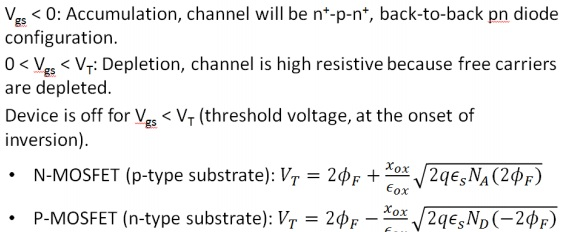
\includegraphics[scale=0.5]{./Images/3/1.jpg}
    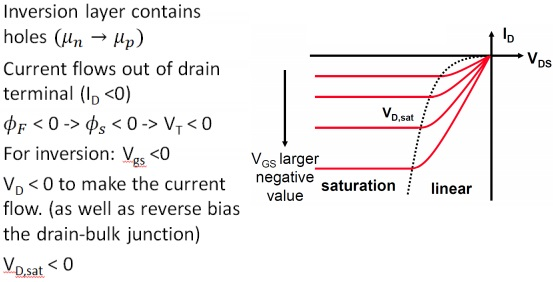
\includegraphics[scale=0.55]{./Images/3/2.jpg}
\end{figure}

Channel Length Modulation
\begin{figure}[H]
    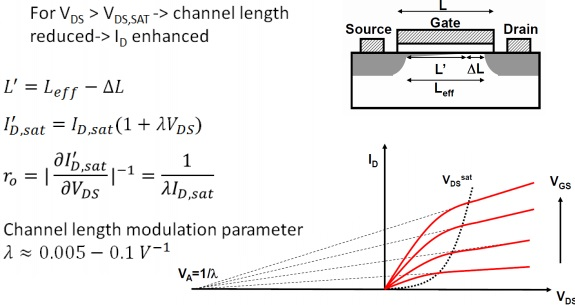
\includegraphics[scale=0.5]{./Images/3/3.jpg}
\end{figure}

Small-Signal Circuit
\begin{figure}[H]
    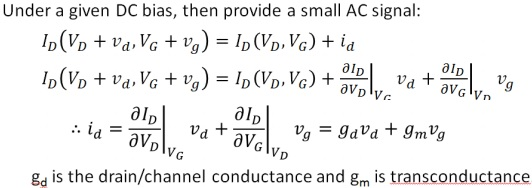
\includegraphics[scale=0.53]{./Images/3/7.jpg}
\end{figure}
Non-Ideal Flat Band, Oxide Charge, Body Effect
\begin{figure}[H]
    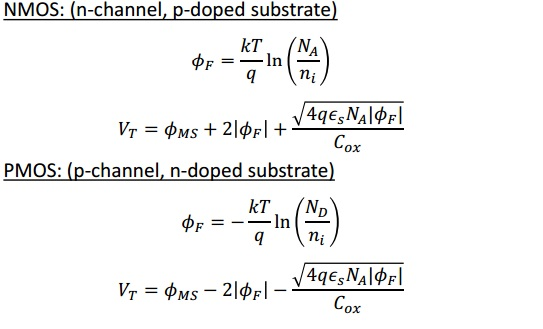
\includegraphics[scale=0.53]{./Images/3/4.jpg}
    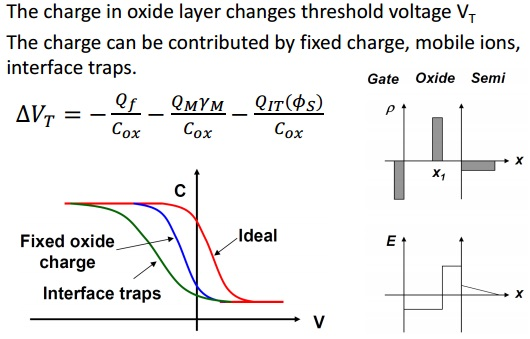
\includegraphics[scale=0.53]{./Images/3/5.jpg}
    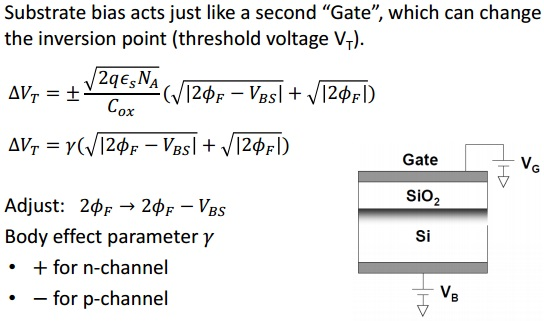
\includegraphics[scale=0.53]{./Images/3/6.jpg}
\end{figure}

C-V
\begin{figure}[H]
    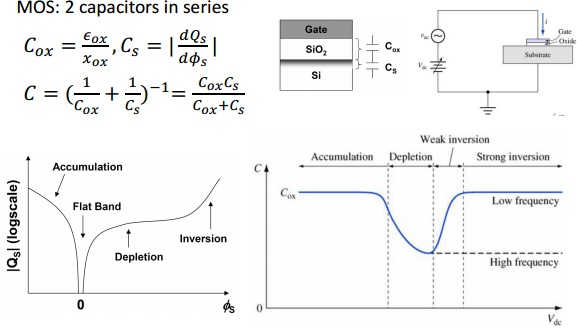
\includegraphics[scale=0.53]{./Images/3/8.jpg}
\end{figure}

BJT Minority Carrier
\begin{figure}[H]
    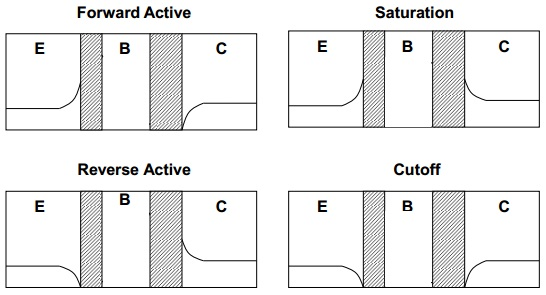
\includegraphics[scale=0.58]{./Images/3/9.jpg}
\end{figure}

BJT Circuit Config
\begin{figure}[H]
    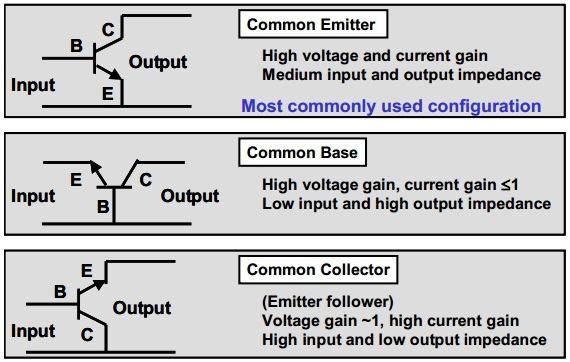
\includegraphics[scale=0.53]{./Images/3/10.jpg}
\end{figure}
\begin{figure}[H]
    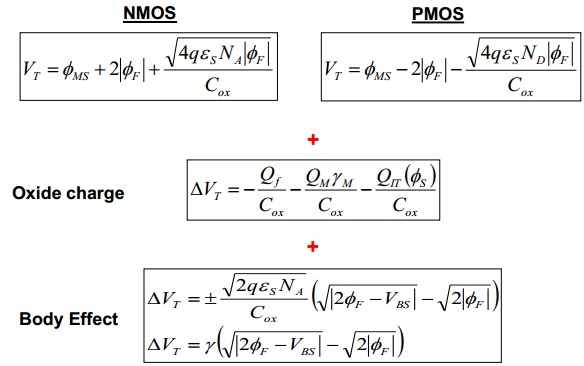
\includegraphics[scale=0.53]{./Images/3/13.jpg}
\end{figure}
\begin{figure}[H]
    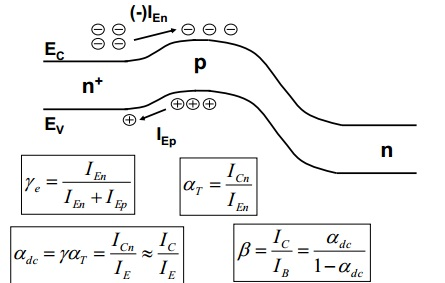
\includegraphics[scale=0.53]{./Images/3/11.jpg}
\end{figure}
\begin{figure}[H]
    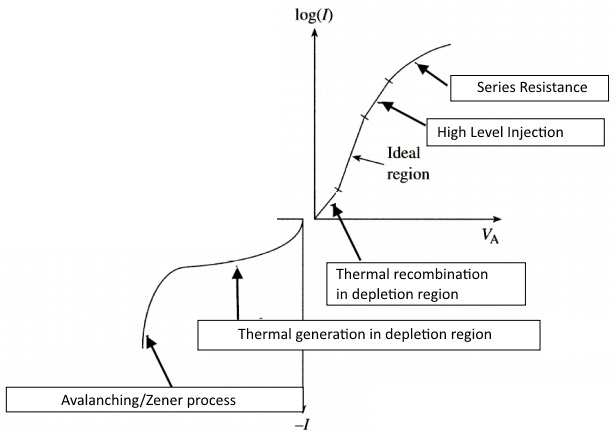
\includegraphics[scale=0.50]{./Images/2/DiodeIV.jpg}
\end{figure}
\begin{figure}[H]
    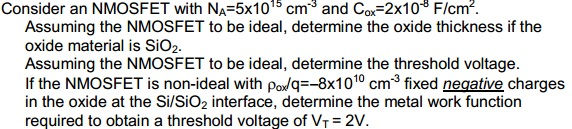
\includegraphics[scale=0.53]{./Images/3/12.jpg}
\end{figure}

\end{multicols}
\end{document}
